% !TEX encoding = UTF-8 Unicode
%!TEX root = thesis.tex
% !TEX spellcheck = en-US
%%=========================================
\section{Methods and implementation}

\subsection{Evolving neural networks}
There are several ways to map sound analysis to effect parameters. The initial idea was a modulation matrix, where each effect parameter becomes a linear combination of the audio features. This idea was quickly iterated upon. Why not use an artificial neural network? An artificial neural network can do the same as a modulation matrix (when the ANN has linear activation functions and no hidden layers), but it can also do more. A neural network can have hidden nodes with various activation functions, which makes more complex signal interactions possible. This widens the scope, and allows for learning higher-level features, such as “the snare and the bass drum are hit simultaneously”.

NEAT (Stanley \& Miikkulainen, 2002) is suggested as a technique for evolving neural networks. This is a technique which evolves not only the weights of the neural network, but also the topology, i.e. the number of nodes and the connections between the nodes. HyperNEAT, a technique that is based on NEAT, has been used with great success in a project called Picbreeder (Secretan et al., 2008) and later with some success in a project called SoundBreeder (Ye \& Chen, 2014). The purpose of those projects were to evolve visually and aurally appealing art, respectively. Since both those two projects and this project are within the field of creative computation, the hypothesis is that NEAT or HyperNEAT will work well in this project.

\subsection{Implementation}
Csound has been selected to be the audio processing tool in this project. Since Csound interoperates nicely with Python, and Python is a popular language for artificial intelligence (AI) applications, that was the language of choice for the neuroevolution application. Further, it has been decided that the application should be written in a style compatible with both Python 2 and 3, for the sake of compatibility with various Python libraries. Also, it should work on both Windows and Ubuntu. This way, experiments can not only run on Windows desktop computers, but also on Ubuntu instances in the cloud. The most important dependency is MultiNEAT (Chervenski \& Ryan, n.d.), which is one of Kenneth Stanley’s recommended neuroevolution libraries (Stanley, n.d.). It features several neuroevolution algorithms, including NEAT, FS-NEAT and HyperNEAT. It is written in C++, but it has Python bindings, so it is fit for this project. Further, the audio features extraction tools selected for this project are Aubio, Essentia and LibXtract, which are all free open source software written in a compiled language. A link to the author’s implementation of the toolkit, which is open source, is included in appendix A. A complete list of dependencies is included in appendix B.

\subsubsection{Performance}
A. Eldhuset has previously implemented a program that uses Csound in signal interaction experiments with genetic algorithms. He concluded that his implementation was slow, taking around 5 seconds per individual (Eldhuset, 2015). Hence an experiment with a population size of 20 and 20 generations would take approximately half an hour. The author has analyzed the weaknesses of Eldhuset's approach and come up with a number of techniques to alleviate performance issues:

\begin{itemize}  
\item Use a templating engine to generate Csound files. It writes csound code to different files, one for each individual in the population. This allows many Csound instances to be run in parallel.
\item While a Csound instance runs, it does not have to communicate with another program (a host) via an API. All data needed for the run, including effect parameter values over time, are included inside the csd file
\item Use dedicated, compiled audio feature extraction tools such as Aubio instead of Csound for audio feature extraction
\item Use the standard streams (stdout) instead of file I/O in audio feature extractors that support this
\item Let the host program, Csound and audio feature extractors write files to a RAM disk to avoid slow disk I/O activity
\item Use the concept of pipelining to shorten critical paths and enable more parallelism
\item Sensible handling of duplicate individuals: when two or more individuals are equal (i.e. their neural networks are equal), evaluate only one of them, and apply the same result to the identical individuals
\end{itemize}

Incorporating all these techniques, the author's implementation spends around 0.11 seconds on average per individual, given that the dist\_lpf effect and the aubio mfcc analyzer is used, the duration of the input sound is 7 seconds, and that the program is run on a modern, high-end laptop with two CPU cores. Hence an experiment with population size 20 and 20 generations may take approximately half a minute.

\subsubsection{Neuroevolution routine}
The neuroevolution program is called from the command line, with a number of arguments for configuring the experiment. The program then performs roughly these steps:

\begin{enumerate}  
\item Check sanity of arguments
\item Analyze input sound file and target sound file
\item Initialize a population
\item For each generation, evaluate all individuals, write their data to json files and then advance to the next generation
\end{enumerate}

The evaluation of an individual involves several operations:

\begin{enumerate}  
\item An artificial neural network is created from the genotype of the individual
\item All feature vectors of the target sound are run through the neural network
\item The neural outputs are scaled to appropriate ranges for the various audio effect parameters
\item Csound runs the input sound through the audio effect that is controlled by the audio effect parameters
\item The resulting sound is run through the audio feature extraction tool(s)
\item The audio features are standardized with the same mean and variance as in the standardization of the target sound audio features
\item The audio features of the target sound and the output sound are used in the fitness function
\item The resulting fitness value is assigned to the individual.
\end{enumerate}

\begin{figure}[h]
    \centering
    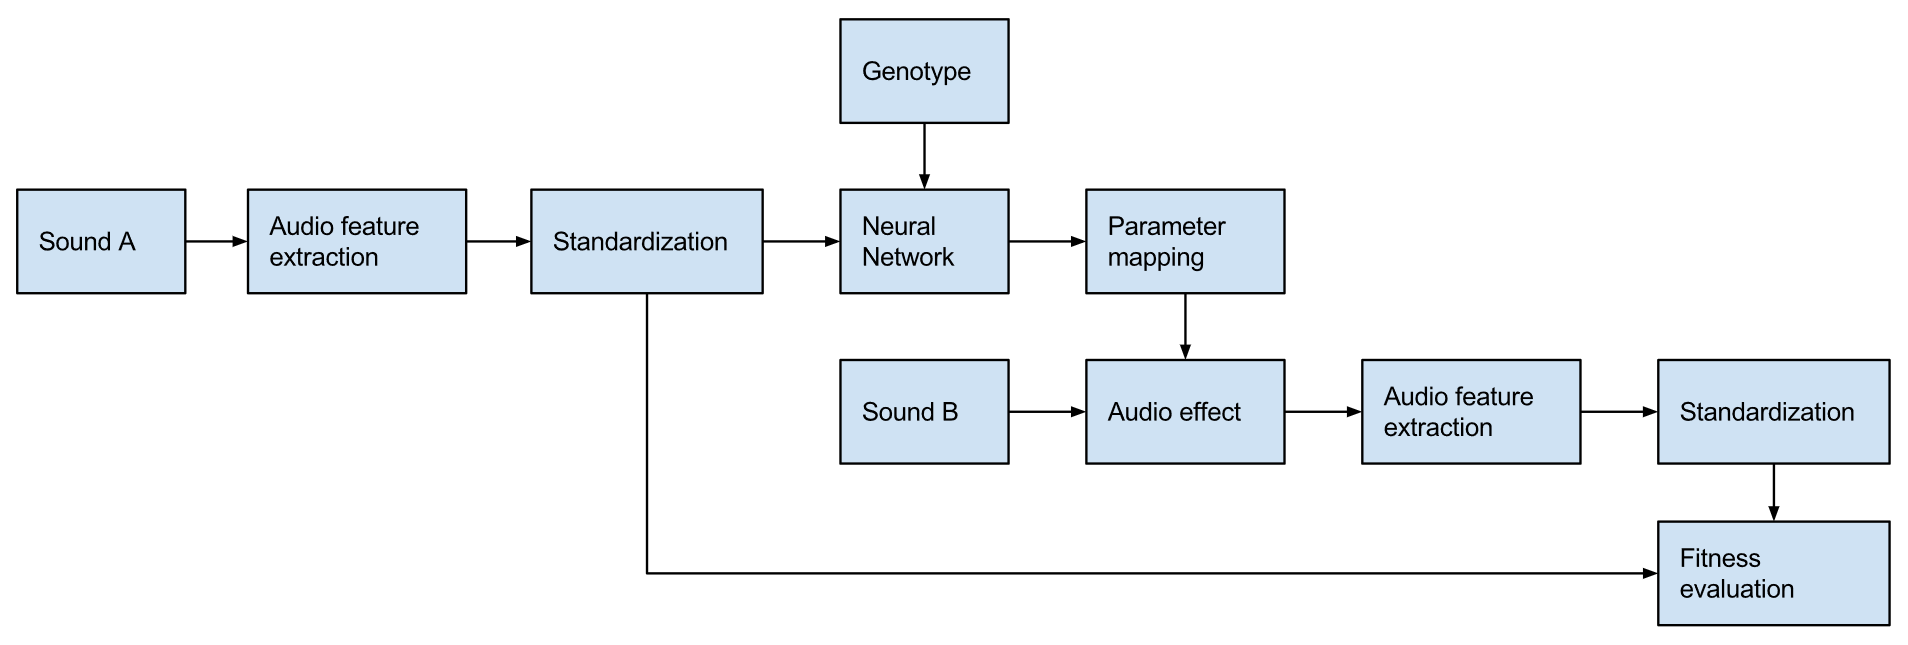
\includegraphics[width=0.99\textwidth]{06_individual_evaluation_process}
    \caption{Flowchart for the evaluation of an individual}
    \label{fig:individual_evaluation_process}
\end{figure}

\subsubsection{Input standardization}
To make the audio features suitable as input to a neural network, they need to be scaled. A simple, but good technique is to standardize them by is subtracting the mean and dividing by the standard deviation (Sarle, 2014). For each audio feature there is one sequence of numbers for the input sound and another sequence for the target sound. The mean and standard deviation for an audio feature is calculated from the input sound’s sequence for that feature concatenated with the target sound’s sequence for that feature. This mean and standard deviation is then used in all further input standardization. This gives the series the quality of being centered around zero and having a standard deviation of 1 with respect to the input sound and the target sound. Additionally, to avoid extreme values, values are clipped to the range [-4, 4].

\subsubsection{Parameter mapping}
The output of the neural network is in the range [0, 1], due to the sigmoid activation function in the output layer. These normalized values need to be scaled and skewed appropriately for each effect parameter. The author has used the same mapping function as in Cabbage (Walsh, 2008), a GUI framework for Csound, where slider values are mapped from 0 to 1 to the target range by the following function:

$$f(x)=m_{min}+(m_{max}-m_{min})*e^{\log(x)/s}$$

Where $m_{min}$ and $m_{max}$ are the endpoints of the target range and s is the skew factor. The default skew factor is 1, which will yield a linear mapping. A skew factor of 0.5 will cause the mapping function to output values in an exponential fashion. This is useful for effect parameters such as cutoff frequency.

\subsection{Visualization}
In very early versions of the neuroevolution program, the author found it hard to evaluate all the data produced during experiments. Therefore an interactive web application for visualizing results was developed. This tool has been very important for being able to understand the strengths and weaknesses of the neuroevolution program during development and research. When the author gained a good understanding of the inner workings and the output of the neuroevolution program, he was able to improve the weak points of the implementation.

The visualization system is a single-page web application written in AngularJS, with various JavaScript libraries for visualizing data. For a complete list of JavaScript libraries that were used in the web application, see appendix C. The application server is written in NodeJS. The neuroevolution program writes data after each generation, and the NodeJS server listens for these data updates. Whenever new data is available, the updated data is sent via WebSockets to the web application, which then updates its views. Figure 3.2 shows a screenshot of how the web application may look.

\begin{figure}[h]
    \centering
    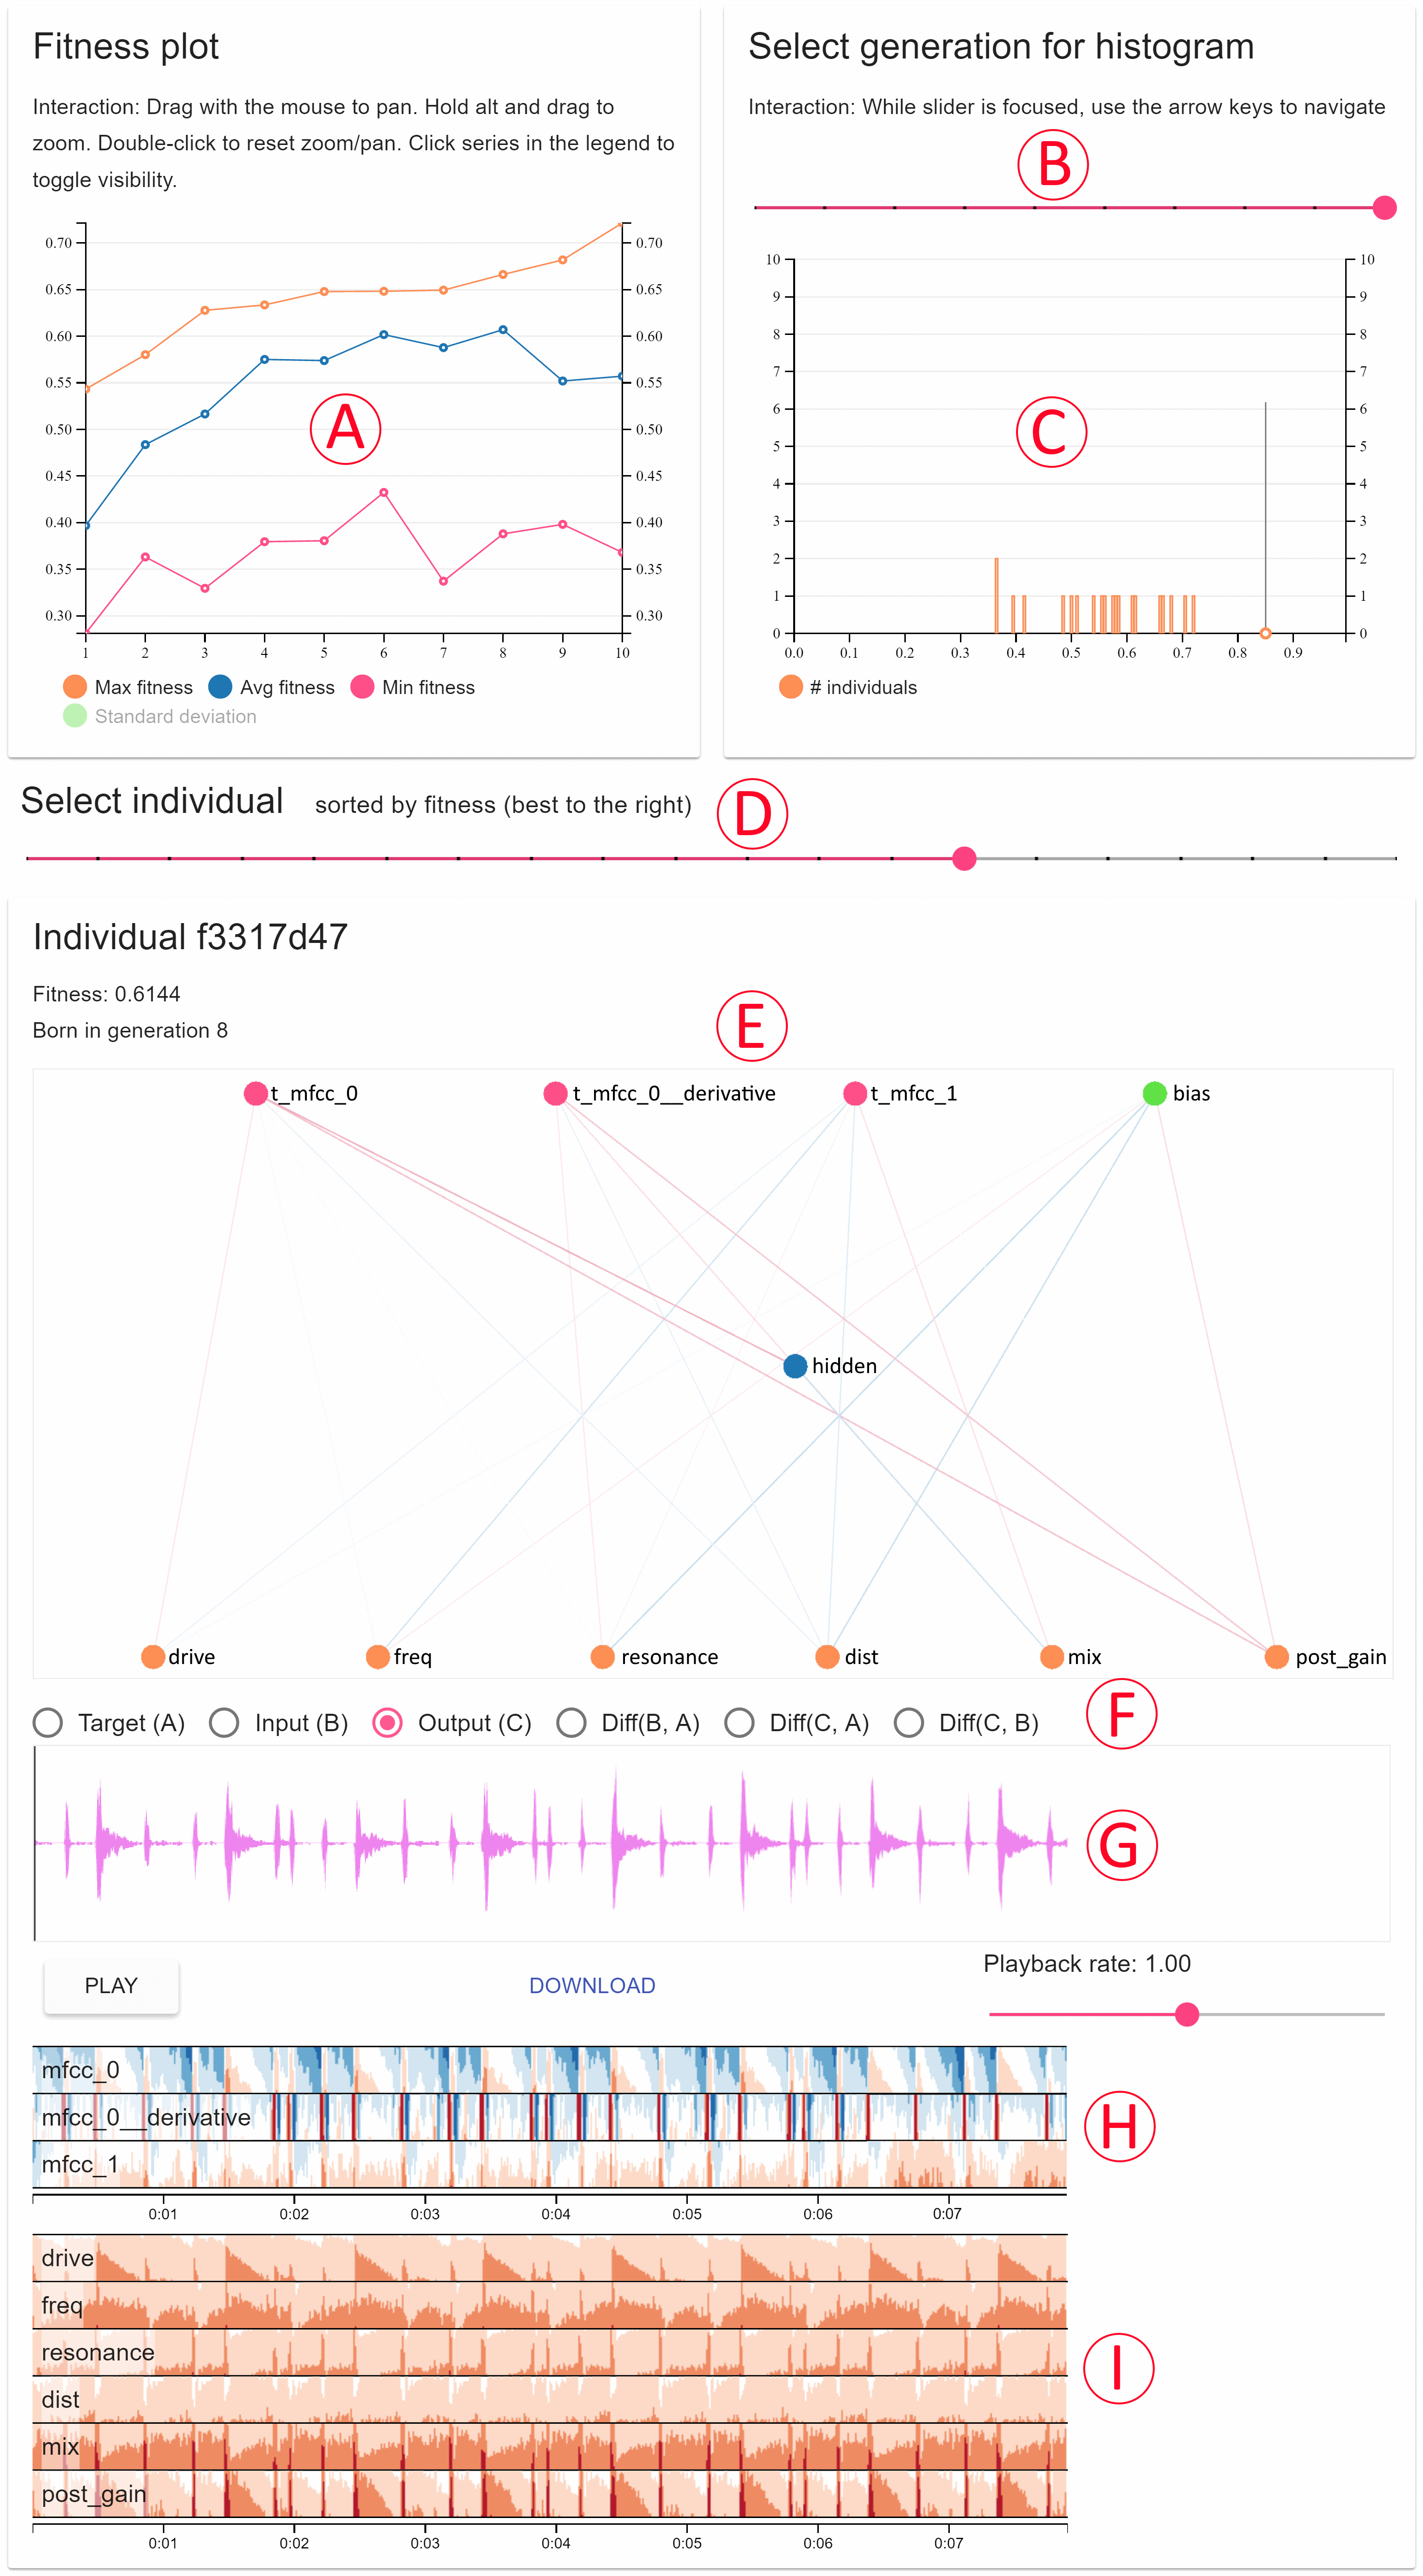
\includegraphics[width=0.99\textwidth]{07_visualization_screenshot_annotated}
    \caption{(TODO: formatting and visibility) Annotated screenshot of the interactive visualization system. A: Fitness plot (line chart, shows the progress of the GA over the generations). B: Interactive slider for selecting a specific generation and visualizing its population. C: Fitness histogram (shows fitness distribution in a population). D: Interactive slider for selecting a specific individual in the population of the selected generation. E: Neural network visualization with edge colors according to weight. Light color means small magnitude while strong color means large magnitude. Red means positive weight while blue means negative. F: Select which sound and corresponding data series to visualize. G: Audio player with waveform visualization. Useful for playing back the output sound of the selected individual. H and I: Horizon charts for visualizing neural input and neural output, respectively. Horizon charts make better use of vertical space than standard area charts, allowing you to see many more metrics at-a-glance. Larger values are overplotted in successively darker colors, while negative values are offset to descend from the top. The horizon charts are aligned with the audio player.}
    \label{fig:visualization_screenshot_annotated}
\end{figure}